\chapter{Reti neurali}
	Per la simulazione della rete neurale della chiocciola, relativa alla sola predizione della marea, ed il conseguente studio della complessità neurale necessaria alla chiocciola per poter eseguire tale predizione con un errore accettabile, si è scelto di iniziare con una \textbf{rete lineare di Widrow}.\\
	Con questa tipologia, molto semplice, di rete neurale si sono ottenuti, come vedremo in maggior dettaglio nei due capitoli successivi, ottimi risultati. Quindi, per quanto concerne la \textit{predizione semplice} e \textit{con errori}, è risultato innecessario avventurarsi nell'utilizzo di reti neurali più complesse.\\
	Tuttavia, per lo studio del problema relativo alla predizione del prossimo picco di alta marea (Capitolo 5) una semplice rete lineare di Widrow non è risultata sufficiente e si è quindi utilizzato un \textbf{Multilayer Perceptron}, ovvero una rete di tipo \textit{Feed-Forward} con un certo numero di neuroni aggiuntivi nello strato nascosto.
	\section{Rete lineare di Widrow}
		La rete di Widrow-Hoff rappresenta una classe di filtri adattivi denominata \textbf{ADALINE} (in un primo momento \textbf{Ada}ptive \textbf{Li}near \textbf{Ne}uron e successivamente \textbf{Ada}ptive \textbf{Lin}ear \textbf{E}lement).\\
		La rete è composta da un unico strato di output ed utilizza una funzione di sommatoria ed una funzione di apprendimento. Ogni input \textit{x} della rete ha un peso \textit{w} associato, quindi l'output corrispondente ad un set di input \(\{x_1, x_2, ...., x_n\)\} è calcolato semplicemente con la media pesata
		\[y = \sum_{j=1}^{n} x_j w_j\]
		\begin{figure}[h]
			\centering
			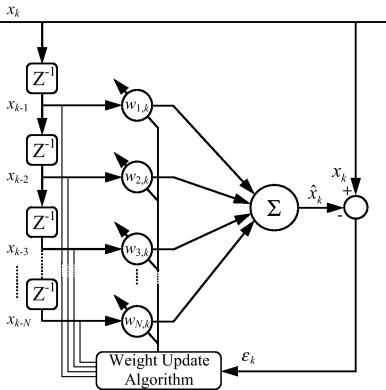
\includegraphics[width=0.4\textwidth]{adaline.jpg}
			\caption{Struttura generica della rete ADALINE}
		\end{figure}
		La struttura risulta quindi molto simile a quella del \textit{Perceptron semplice} e, più in generale, al modello neurale di McCulloch-Pitts, tuttavia differisce per la funzione di apprendimento: l'algoritmo di apprendimento di Widrow-Hoff (anche detto \textbf{\(\alpha-LMS\)}) aggiorna, ad ogni iterazione, i pesi in base alla media pesata degli input. Indicando con \(\textit{t}_k\) l'output atteso (target) al passo \textit{k}, \(\textit{y}_k\) l'output ottenuto al passo \textit{k}, \(\textit{x}_k\) e \(\textit{w}_k\), rispettivamente, il vettore di input ed il vettore di pesi al passo \textit{k} e \textit{\(\alpha\)} un parametro che regola la velocità di convergenza del metodo (detto anche \textbf{learning rate}), allora l'algoritmo di apprendimento risulta
		\[w_{k+1} = w_k + \alpha(t_k - y_k)\frac{x_k}{|x_k|^2}\]
		che, quindi, prescinde dall'appartenenza ad una classe come il Perceptron standard (ricordiamo che la regola di apprendimento del perceptron doveva innanzitutto capire come doveva essere classificato l'output e come era effettivamente classificato, in 1 o -1, e quindi aggiornare i pesi di conseguenza) ed inoltre normalizza l'input in modo automatico.\\
		Quindi risulta che la rete lineare di Widrow converge più velocemente del Perceptron ed inoltre  riesce a risolvere problemi di calcolo che il Perceptron, che si limita ad una semplice classificazione binaria, non può risolvere.\\
		\begin{figure}[h]
			\begin{center}
				\setlength\fboxsep{0pt}
				\setlength\fboxrule{2pt}
				\fbox{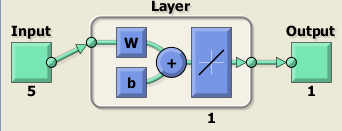
\includegraphics[width=0.5\textwidth]{structure_linear.png}}
			\end{center}
			\caption{Struttura della rete utilizzata per la simulazione in MatLab}
		\end{figure}\\
		La rete utilizzata in MatLab per questo studio corrisponde al comando \textit{newlin}, che prende in input una matrice NxM di \textit{M} vettori di input (per l'addestramento), ognuno dei quali composto da \textit{N} elementi, una matrice KxM di \textit{M} output target, ognuno di \textit{K} elementi, un vettore di ritardi, non utilizzato per questo progetto, ed il parametro di \textit{learning rate}, impostato a \textbf{0.01}.\\
		La rete è stata addestrata su \textbf{20000} input, per la predizione semplice e con errori, e \textbf{10000} input, per la predizione della prossima alta marea; ognuno dei quali composto da \textbf{5 orari} a distanza prefissata, distribuiti casualmente nell'arco di \textbf{28 giorni}.
		
	\section{Multilayer Perceptron}
		Il Multilayer Perceptron rappresenta, come si può intuire, la naturale evoluzione del Perceptron standard. Esso fu ideato da Rumelhart et al. e consiste nell'aggiungere al Perceptron semplice uno o più \textbf{strati intermedi} (o \textbf{nascosti}) di neuroni tra lo strato di input e quello di output.\\
		Il grande vantaggio del Multilayer Perceptron rispetto al Perceptron standard è di poter risolvere anche problemi non lineari e quindi di poter essere applicato a quei problemi che il Perceptron semplice non potrebbe risolvere (come ad esempio il problema dello XOR): in altre parole, il Multilayer Perceptron riuscì a superare le limitazioni che Minsky e Papert individuarono nello studio del Perceptron lineare.\\
		Ogni strato nascosto può utilizzare una funzione di trasferimento diversa dalla semplice \(\Theta\), detta \textit{theta di Heaviside}, che assume soltanto i valori binari 0 ed 1: ad esempio una scelta molto comune è una particolare \textit{funzione sigmoidale} detta \textbf{funzione logistica}, per la quale vale
		\[logsig(x) = \frac{1+\tanh(x)}{2}\]
		con \(logsig(x)\) funzione sigmoidale rispetto ad \textit{x} e \(\tanh(x)\) tangente iperbolica rispetto ad \textit{x}.\\
		\begin{figure}[h]
			\centering
			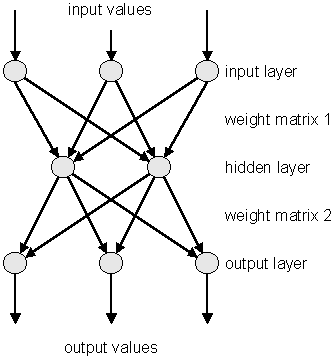
\includegraphics[width=0.5\textwidth]{multi.png}
			\caption{Multilayer Perceptron con 3 input, 3 output e 2 neuroni nello strato nascosto}
		\end{figure}\\
		Il metodo di apprendimento del Multilayer Perceptron è una regola chiamata \textbf{Backpropagation} in quanto, durante l'apprendimento, per ogni pattern di input esaminato (cioè ogni \textbf{epoca}), i pesi vengono aggiornati dallo strato di output verso lo strato di input. Al contrario, il metodo utilizzato dalla rete per produrre un output viene detto di \textbf{Feed-Forward} in quanto i segnali passano dallo stato di input verso quello di output.\\
		\begin{figure}[h]
			\begin{center}
				\setlength\fboxsep{0pt}
				\setlength\fboxrule{2pt}
				\fbox{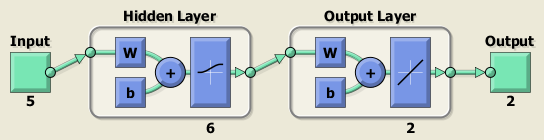
\includegraphics[width=0.7\textwidth]{structure_ff.png}}
			\end{center}
			\caption{Struttura del Multilayer Perceptron utilizzato in MatLab}
		\end{figure}\\
		In MatLab questo tipo di rete viene creato richiamando la funzione \textit{newff}, la quale richiede come parametri una matrice di input, una matrice di output, una vettore con indicato il numero di neuroni presenti negli (eventuali) strati nascosti, una lista delle funzioni di trasferimento per ogni strato (dal primo strato nascosto fino allo strato di input) ed, eventualmente, la funzione di apprendimento.\\
		Nelle simulazioni effettuate con questa rete si è utilizzato un Multilayer Perceptron con uno strato nascosto composto da \textbf{6 neuroni}; le funzioni di trasferimento utilizzate sono \textbf{logsig}, ovvero la funzione logistica, per lo strato nascosto, e \textbf{purelin}, cioè la funzione di trasferimento lineare, per lo strato di output. La funzione di apprendimento utilizzata in questo caso è \textbf{trainlm}, che corrisponde alla regola di Backpropagation di Levenberg-Marquardt.\\
		L'apprendimento della rete è stato effettuato su \textbf{10000} gruppi di orari, ognuno composto da \textbf{5 ore} a distanza di \textbf{1 ora}.